% !Mode:: "TeX:UTF-8" 

\chapter{\hei 实验测试}

\section{\hei 实验背景}
Python 的 sklearn扩展包中包含了“威斯康星州乳腺癌”数据集,其中详细记录了威斯康星大学附属医院的乳腺癌测量数据。数据集包括 569 行和 31 个特征。 可以使用这个数据集训练一个支持向量机模型,以判断一个患者的肿瘤是良性还是恶性。

\section{\hei 实验步骤}
\begin{itemize}
    \item 加载data文件夹里的数据集:威斯康星乳腺肿瘤数据集
    \item 进行数据清洗(如删除无用列,将诊断结果的字符标识B、M替换为数值0、1等)
    \item 进行特征选取(方便后续的模型训练)。
    \item 进行数据集的划分(训练集和测试集),抽取特征选择的数值作为训练和测试数据。
    \item 配置模型,创建SVM分类器,选取线性核函数与高斯核函数进行对比。
    \item 训练测试与评估模型。
\end{itemize}

\section{\hei 实验结果}
\begin{equation*}
\begin{aligned}
    Accuracy \ of \ Linear \ kernel: \ 95.32\%  \\
Accuracy \ of \ RBF \ kernel: \ 94.74\%
\end{aligned}
\end{equation*}

\begin{figure}[!h]
	\centering
	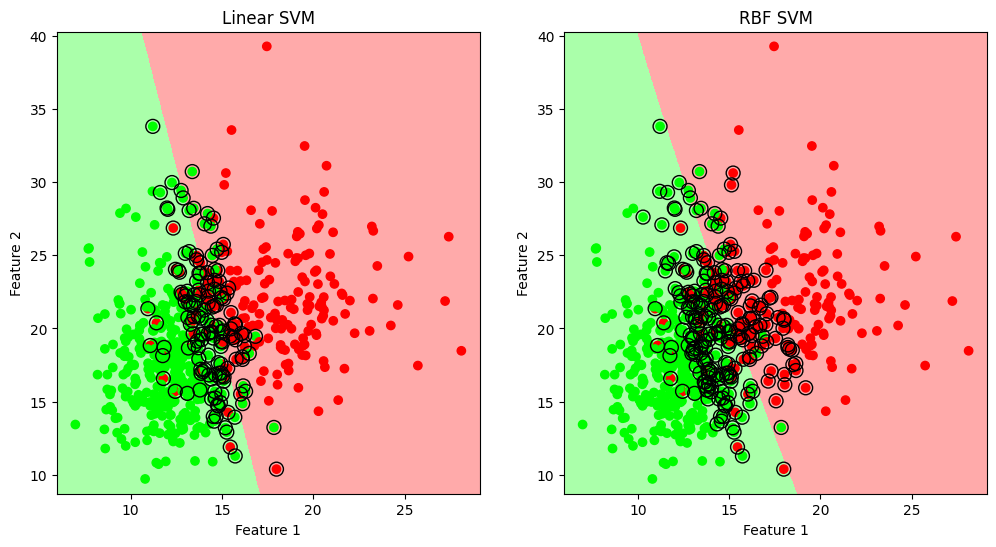
\includegraphics[scale=0.4]{download.png}
	\caption{线性核函数与高斯核函数相对比}
	\label{bfgs}
\end{figure}
{\hei 实验结果表明,高斯核函数在本数据集上的表现优于线性核函数,具有更高的准确率,这说明高斯核函数能够更好地捕捉数据的非线性特征,提高分类性能。}

\chapter{\hei 支持向量机算法的应用}
支持向量机算法可以有效地处理高维数据和非线性数据,具有很高的准确性和泛化能力,在模式识别、生物信息学、金融预测、医学检测、计算机视觉、文本分类等领域都有广泛应用。
\section{\hei 模式识别}
支持向量机在模式识别领域的应用最广泛,已成功地解决了诸如手写体、图像处理、语音识别等许多识别和分类问题。

在手写字体识别方面,当采用5层神经网络算法时,其识别的错误率为5.1\%;贝尔实验室\cite{cortes1995support}最先将SVM应用于手写字体识别研究,选取三种不同的核函数时,得到的误识率分别为4.0\%,4.1\%和4.2\%,可看出支持向量机方法比神经网络算法具 有更好的分类准确性。

在人脸识别方面,使用C-SVC和nu-SVC支持向量机模型,对人脸进行识别,在叶晓波等\cite{叶晓波2019基于支持向量机的人脸识别应用研究}的实验验结果显示,nu-SVC模型的人脸识别正确率高,且波动性小,更适合用于人脸识别,SVM分类器用于人脸识别效果较好。

在语音识别方面,由于背景环境中存在不同程度的噪杂声,熊卫华\cite{熊卫华2018基于最小二乘支持向量机的含噪语音识别算法}等设计了一种基于集总经验模态分解(EEMD)和最小二乘支持向量机(LSSVM)的语音识别算法,该方法能够快速有效地识别各种语音信号,与EEMD结合BP神经网络方法相比,识别准确率更高,抗干扰能力更强。

\section{\hei 金融预测}
随着经济水平的提高,越来越多的人投入到了股票预测的研究之中,在众多的股票预测方法中,支持向量机对于回归预测也有很强大的效果。张磊\cite{张磊2020基于支持向量机的股票市场趋势分析及预测研究}通过主成分分析降维,让支持向量机模型在略微的预测正确率损失情况下其运行速度得到巨大的提升,同时发现支持向量机对于预测股票的最佳时间滑窗为3,支持向量分类和回归的结合能提升模型3\%-4\%的预测准确率。

\section{\hei 文本分类}
利用计算处理系统处理文本信息,能够有效提升文本分类的质量与效率,提升数据信息的利用率,从而促进信息化技术的普及\cite{何焱2019文本分类中支持向量机研究}。何铠等\cite{何铠2022基于深度学习和支持向量机的文本分类模型}在传统卷积神经网络模型的基础上提出了一种基于卷积神经网络和支持向量机结合的文本分类模型CNNSVM,使用基于支持向量机的分类器替代传统模型中的softmax层帮助实现文本的分类。该模型提升了特征词语的提取效果,有效解决了softmax层泛化能力较弱的问题。

\chapter{\hei 结论与展望}
SVM 以统计学习理论为基础,存在全局优化、泛化性能好等优点,同时也存在诸多缺陷,有很多问题需深入研究:
\begin{enumerate}
    \item SVM算法对大规模训练样本难以实施,这是因为支持向量算法借助二次规划求解支持向量,这其中会设计m阶矩阵的计算,所以矩阵阶数很大时将耗费大量的机器内存和运算时间。这也限制了SVM在大数据领域的应用。
    \item SVM对非线性问题没有通用解决方案,有时候很难找到一个合适的核函数。核函数的选择需要根据数据的特点和经验进行调整,没有一个统一的标准。核函数的选择也会影响SVM的性能和效果。
    \item SVM对缺失数据敏感,对参数和核函数的选择敏感。SVM需要对数据进行预处理,如归一化、去噪等,否则会影响分类结果。SVM的参数如正则化参数C、核函数参数gamma等也需要通过交叉验证等方法进行调优,否则会导致过拟合或欠拟合。
    \item SVM的模型解释性不强,难以理解为什么会做出某种预测。SVM的模型涉及到高维空间的映射和超平面的构造,不容易直观地展示给用户。SVM也没有提供特征选择或权重分配的方法,不容易分析特征对分类结果的影响。
\end{enumerate}

目前,SVM 仍然存在很多问题需进一步的研究,可将SVM与离散余弦变换、小波包分解、主元分析、独立分量分析、聚类、粗糙集理论、深度神经网络等方法结合\cite{张松兰2016支持向量机的算法及应用综述},提高应用效果并不断探索SVM新的应用领域。